\subsubsection{\stid{3.06} PETSc-TAO} \label{subsubsect:petsc}
\paragraph{Overview} 

Algebraic solvers (generally nonlinear solvers that use sparse linear solvers via Newton's method) and ODE/DAE 
integrators form the core computation of many numerical simulations. No scalable ``black box'' sparse solvers 
or integrators work for all applications, nor single implementations that work well for all scales of 
problem size. Hence, algebraic solver packages provide a wide variety of algorithms and implementations 
that can be customized for the application and range of problem sizes at hand. PETSc~\cite{petsc:homepage,petsc-man} 
is a widely used software library for the scalable solution of linear, nonlinear, and ODE/DAE systems and 
computation of adjoints (sometimes called sensitivities) of ODE systems. We focus on three topics: (1) partially 
matrix-free scalable solvers efficiently use many-core and GPU-based systems; (2) reduced synchronization 
algorithms that can scale to larger concurrency than solvers with synchronization points; and (3) performance 
and data structure optimizations for all the core data structures to better utilize many-core and GPU-based 
systems as well as provide scalability to the Exascale.

The availability of systems with over 100 times the processing power of today's machines compels the utilization 
of these systems not just for a single ``forward solve'' simulation (as discussed above) but rather within a 
tight loop of optimization, sensitivity analysis (SA), and uncertain quantification (UQ). This requires the 
implementation of a new, scalable library for managing a dynamic hierarchical collection of running scalable simulations, where the simulations directly feed results into the optimization, SA, and UQ solvers.  This library, 
which we call libEnsemble, directs the multiple concurrent ``function evaluations'' through the tight coupling 
and feedback described above. This work consist of two parts: (1) the development of libEnsemble and (2) the 
extension of TAO~\cite{tao-man} (our PETSc-based scalable optimization library) with new algorithms and 
software to utilize libEnsemble.

\paragraph{Key Challenges}

A key challenge for for scaling the PETSc/TAO numerical libraries to Exascale systems is that 
traditional ``sparse-matrix-based'' techniques for linear, nonlinear, and ODE solvers, as well 
as optimization algorithms, are memory-bandwidth limited.  Another difficulty is that any 
synchronizations required across all compute units--for example, an inner product or a 
norm--can dramatically affect the scaling of the solvers.

Running an ensemble of simulation requires a coordination layer that handles load balancing and
allows the collection of running simulations to grow and shrink based on feedback. Thus, this 
library must be able to dynamically start simulations with different parameters, resume 
simulations to obtain more accurate results, prune running simulations that the solvers 
determine can no longer provide useful information, monitor the progress of the simulations, 
and stop failed or hung simulations, and collect data from the individual simulations both 
while they are running and at the end.

\paragraph{Solution Strategy}

To address the scalability of the numerical libraries, we are developing new solvers and data 
structures including pipeline Krylov methods that delay the use of the results of inner products 
and norms, allowing overlapping of the reductions and other computation; partially matrix-free 
solvers using high-order methods that have high floating-point-to-memory-access ratios and
good potential to use many-core and GPU-based systems; and in-node optimizations of sparse 
matrix-matrix products needed by algebraic multigrid to better utilize many-core systems
using a thread neutral ``bypass MPI'' approach, which implements default interprocessor 
communication using MPI but bypasses the use of MPI in performance-critical regions 
for higher performance and thereby maintains MPI portability.

Our strategy for coordinating ensemble computations has been to develop libEnsemble
to satisfy our needs.  This library should not be confused with workflow-based 
scripting systems; rather it is a library that, through the tight coupling and 
feedback described above, directs the multiple concurrent ``function evaluations''
needed by optimization, SA, and UQ solvers.

\paragraph{Recent Progress}

In the past year, we have released PETSc 3.9 (available at \url{http://www.mcs.anl.gov/petsc})
that features pipeline Krylov implementations and improved performance on SIMD
architectures.  Performance at scale on Theta at Argonne for a 2-D reaction 
diffusion example on a 16384x16384 mesh using a multigrid preconditioner with 
6 levels is shown in Figure~\ref{fig:petsc-tao-fig}. The SIMD optimization 
delivers 2x faster matrix multiply, while not obviously slowing down other 
kernels.  The effect of better vectorization is minimal when available 
memory bandwidth is low.

\begin{figure}
\centering
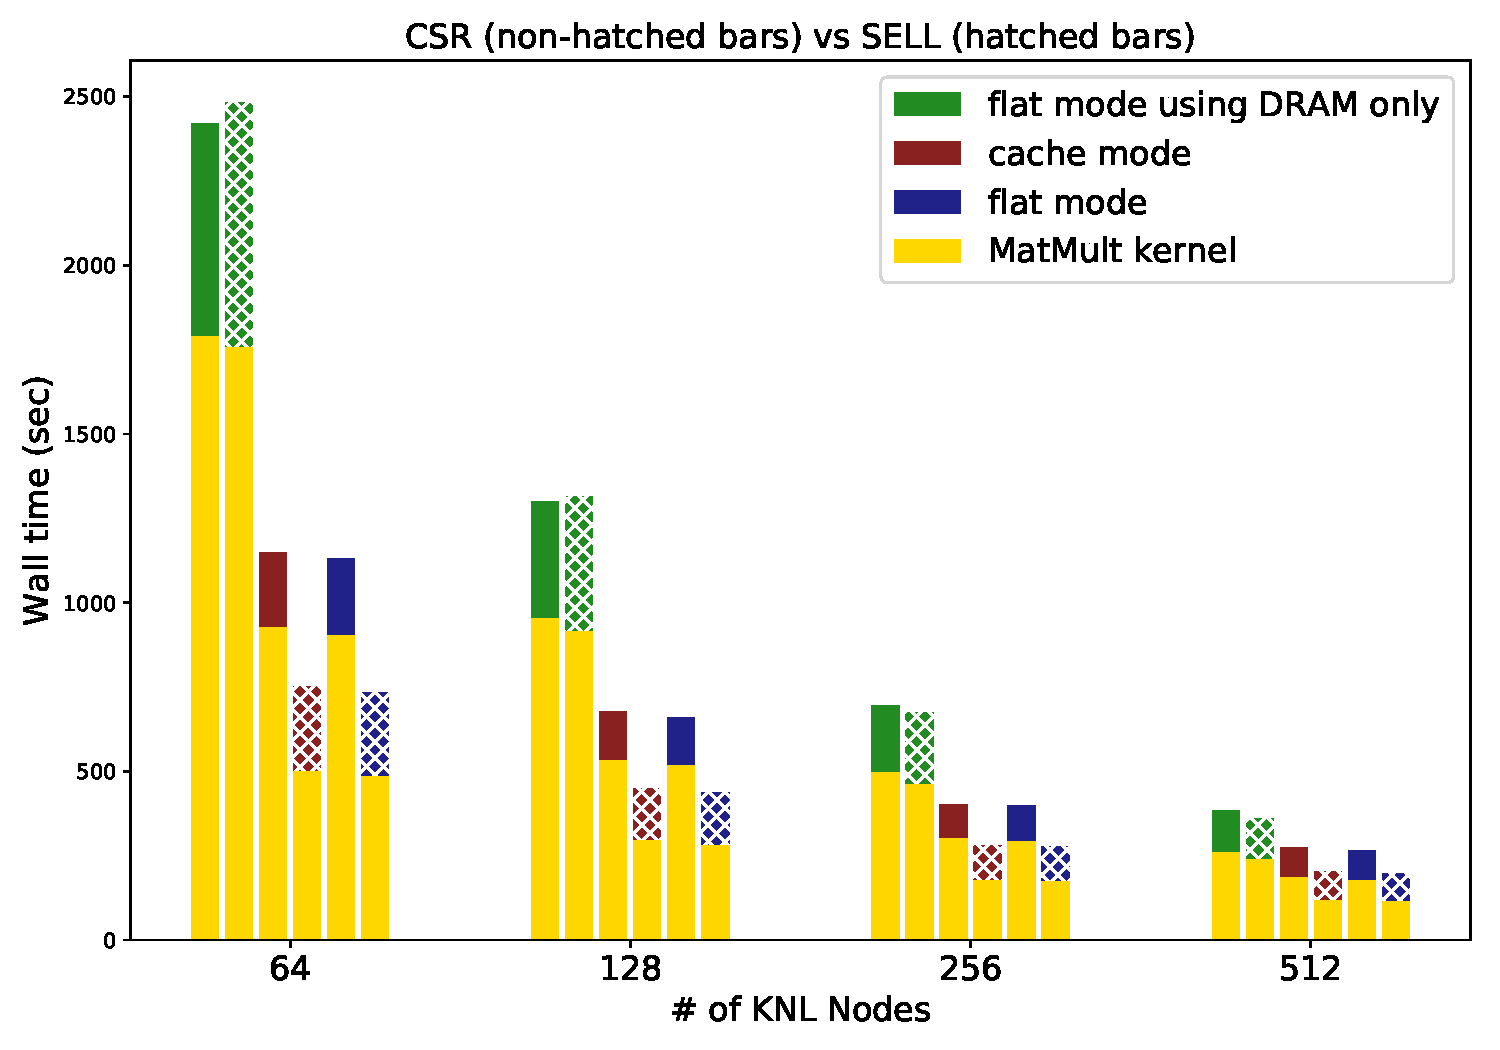
\includegraphics[width=0.5\textwidth]{projects/2.3.3-MathLibs/2.3.3.06-PETSc-TAO/aij_vs_sell}
\caption{Performance at scale on Theta at Argonne for a 2-D reaction diffusion 
example on a 16384x16384 mesh using a multigrid preconditioner with 
6 levels.}
\label{fig:petsc-tao-fig}
\end{figure}

We have also developed the libEnsemble API, implemented it in Python, released 
version 0.1.0 (available at \url{https://github.com/Libensemble/libensemble}),
and provided a Spack installation.  The code has been testing using the
POUNDERS numerical optimization solver.

\paragraph{Next Steps}

Our next efforts are:
\begin{enumerate}
  \item \textbf{Release libEnsemble with monitoring and pools}: Incorporate improved scheduling 
    and basic online monitoring into libEnsemble with a dynamic pool of simulations.  This will
    be the first supported release.
  \item \textbf{Release PETSc with enhanced GPU support}: Release of PETSc with enhanced GPU 
    support specifically developed and optimized anticipated architectures.
\end{enumerate}

